\section{Test results\label{sec:results}}

To test the efficacy of the method, a first study of meson and baryon two-point
correlators was
performed. In addition, the method is demonstrated for a two-meson system.
The background gauge fields were generated by the {\em Hadron
Spectrum Collaboration} \cite{Edwards:2008ja,Lin:2008pr}. They are $16^3 \times 128$
and $20^3 \times 128$ anisotropic lattices, with the ratio of spatial to
temporal lattice spacings $a_s/a_t=3.5$ and 2+1 flavors of dynamical quarks.
The bare light-quark mass is $a_t m_q=-0.0840$, and when the $\Omega$ baryon
mass is used to set the scale, the corresponding pion mass is $383$ MeV.
The valence-quark action is the same as the light-dynamical-quark
action.

The numerical techniques for the iterative solution of the sparse linear system
for the Sheikholeslami-Wohlert improved discretisation of the Dirac equation
are described in Ref.~\cite{Edwards:2008ja}.  In particular, the EigCG
inverter~\cite{Stathopoulos:2007zi} was used for the solution of these linear
systems.
This method uses eigenvector deflation to accelerate convergence.
The first few inversion calls are needed to construct a sufficient basis, and
subsequent inversions are accelerated by a factor of about three or more
compared to the undeflated solver. For the lattices considered here, this
asymptotic rate is found for $N\ge 4$.
\label{subsec:results-intro}

\subsection{The profile of the distillation operator}
    \label{subsec:results-wavefn}

The distillation operator is written as a low-rank projection operator into a
vector space of smooth fields. As such, there is little physical intuition to
suggest it resembles more traditional smearing algorithms in generating a field
that is roughly localized in some confining region while still remaining
smooth. To examine the properties of the operator, its spatial distribution
was computed. Defining
\beq
   \Psi(r) = \sum_{x,t} \sqrt{\mbox{Tr } \left(\Box_{x,x+r}(t) \Box_{x+r,x}(t)
       \right)},
\eeq
means $\Psi$ is a gauge-invariant measure of the degree to which a field is
smeared by the application of the distillation operator.
\begin{figure}[h]
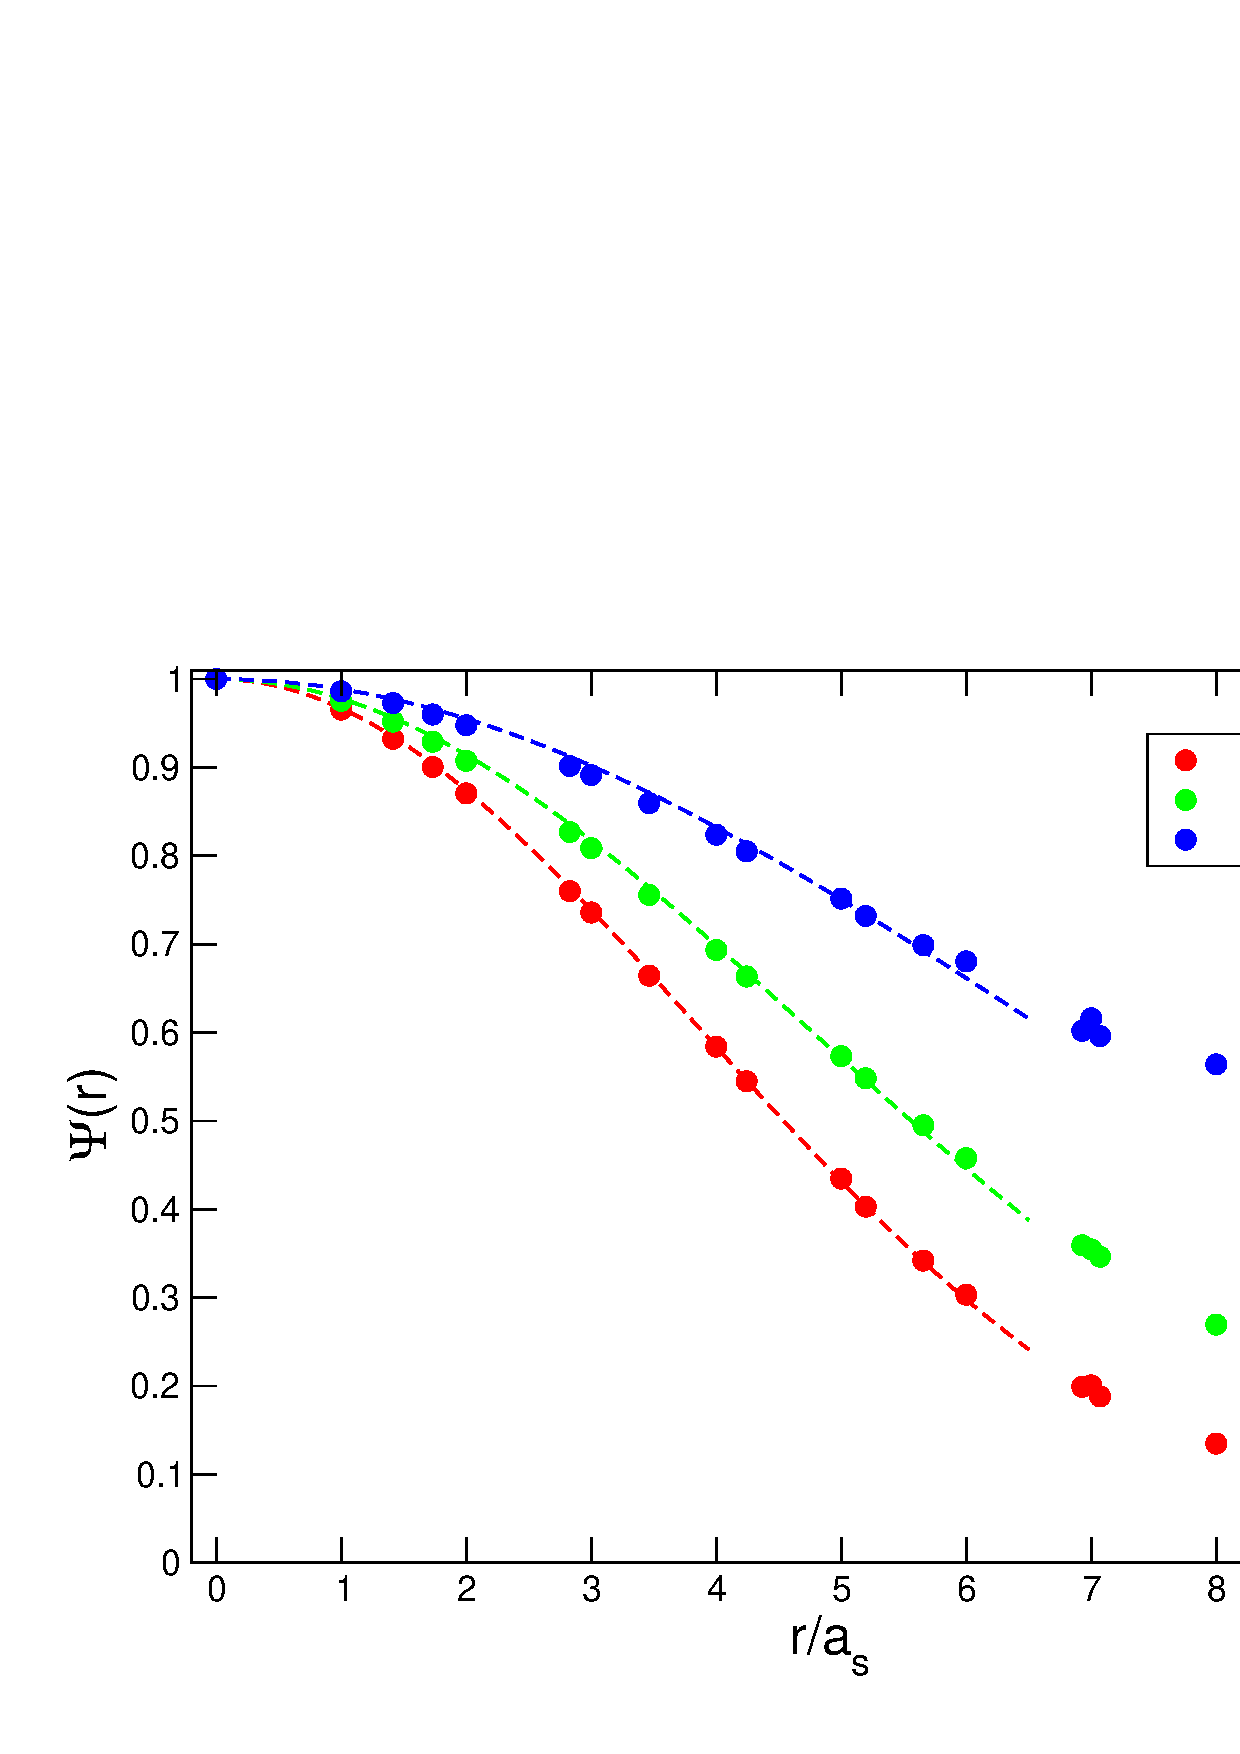
\includegraphics[width=0.6\textwidth]{images/wavefn.pdf}
\caption{\label{fig:wavefn} The spatial distribution of the distillation
  operator constructed from the lowest eigenvalues of the Laplace operator on
    the lattice. Data is from a $20^3$ spatial volume and statistical
    fluctuations are much smaller than plot symbols. The dashed lines are
    fits to a gaussian distribution.}
\end{figure}
This observable was measured for various values of $N$ and for a range of
different off-set vectors $r$ on a small ensemble of the $20^3$ spatial
lattices and the results are
presented in Figure~\ref{fig:wavefn}. The data clearly shows that for $N$
between 8 and 64 the distillation operator is very
well described by a gaussian wavefunction. As $N$ increases, so the radius of
this distribution reduces. This behaviour is to be anticipated since when $N=M$
the distillation operator is the identity and has no spatial extent at all.
The measurements presented in Fig.~\ref{fig:wavefn} also clearly illustrate
the distillation operator has good rotational symmetry, indicating it
is only very weakly influenced by dynamics at the lattice cut-off. The artifacts
seen at larger values of $r$ in the very broad $N=8$ distribution arise solely
from the finite lattice volume used in these measurements.

\subsection{Meson correlation functions}\label{subsec:results-mesons}

In this section, connected meson correlation functions formed using the
derivative-based operators presented in Refs.~\cite{Liao:2002rj,Dudek:2007wv}
are shown, with particular focus on the $T_1^{--}$ channel.
Fig~\ref{meff} shows plots of the effective mass, defined by
\begin{equation}
m_{\mathrm{eff}}(t) = - \frac{1}{\delta t} \ln \left(\frac{C(t+\delta t)}{C(t)}\right)
\end{equation}
with $\delta t = 5 a_t$, for four diagonal correlators while varying the
number of distillation vectors. Also shown are the corresponding effective
masses computed using the traditional point-to-all propagator construction
with both unsmeared and Jacobi-smeared sources. The four operators used are
defined in Table \ref{optab}. In all cases, gauge links in the operators are
stout-smeared~\cite{Morningstar:2003gk}. 90 configurations of the
$16^3 \times 128$ lattice were used for this comparison.
\begin{figure*}
 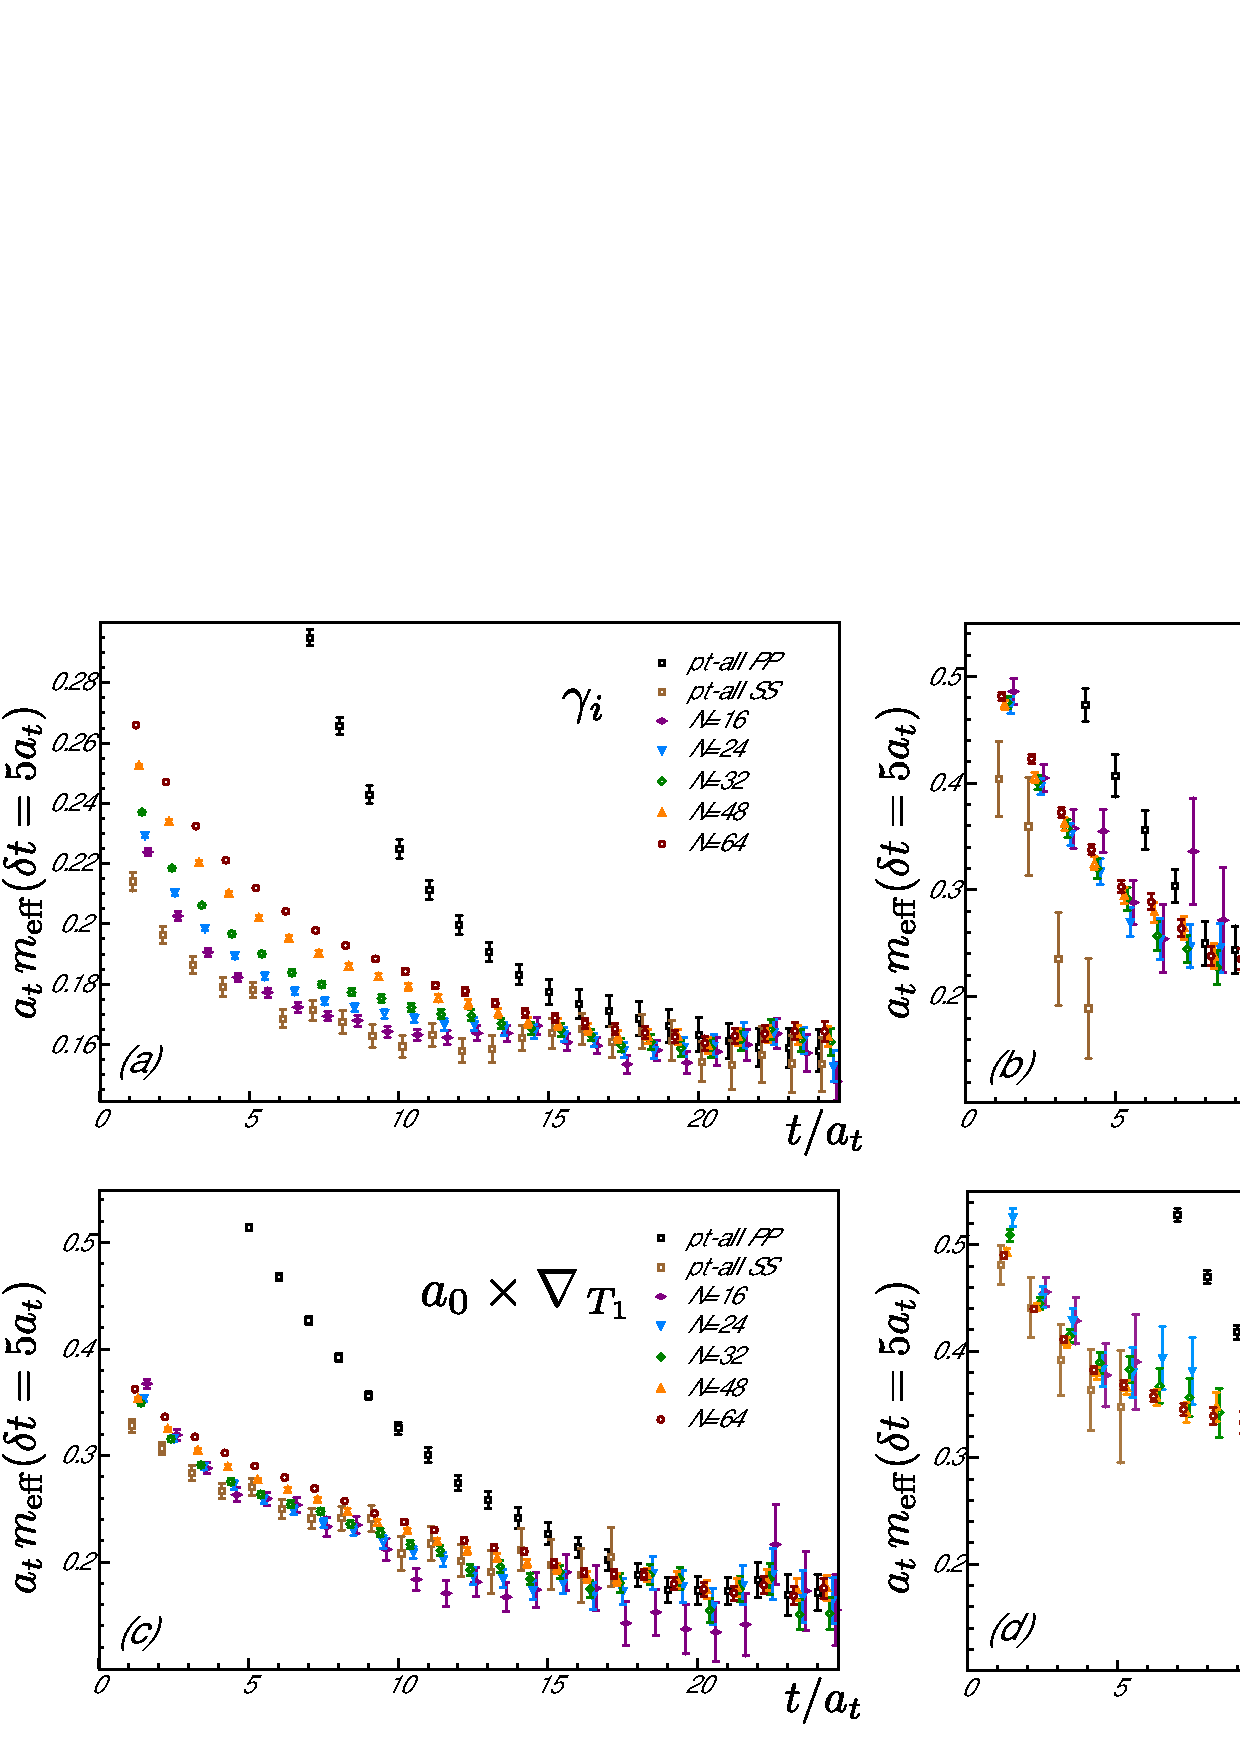
\includegraphics[width=16cm]{images/combined_notrans.pdf}
\caption{\label{meff} Effective masses (five timeslice shift) for diagonal
  correlators in the
$T_1^{--}$ channel computed on $16^3\times 128$ lattices. The operator
construction is shown in table \protect \ref{optab}. Correlators are
constructed using distilled quark fields with $N \in \{16,24,32,48,64\}$ vectors
and using point-to-all methods with standard gauge-invariant quark smearing
(SS, brown) and without (PP, black). }
\end{figure*}
\begin{table}
 \begin{tabular}{c | c}
Name & Construction\\
\hline
$\gamma_i$ & $\bar{\psi}\gamma_i\psi$ \\
$a_0\times \nabla_{T_1}$ & $ \bar{\psi} \nabla_i \psi$ \\
$\rho \times \mathbb{D}_{T_1}$ & $ |\epsilon_{ijk}|\, |\epsilon_{klm}|\,  \bar{\psi} \gamma_j  \nabla_l \nabla_m\psi$\\
$\pi \times \mathbb{B}_{T_1}$ & $ \epsilon_{ijk} \, \bar{\psi} \gamma_5 \nabla_j \nabla_k \psi$
\end{tabular}
\caption{\label{optab}Derivative-based meson operators used in these tests.
  $\vec{\nabla}$ is the one-link discretised covariant derivative}
\end{table}

A variational analysis \cite{Michael:1985ne,Luscher:1990ck} of matrices of
two-point correlation functions has proven to be a powerful method in
extracting the spectrum and matrix elements of excited states
\cite{Dudek:2006ej}. Consequently, cost estimates in terms of the computing
time required to form such a matrix of correlators and not just any single
correlator should be considered.
As a measure of the relative computational demands of distillation versus the
traditional point-to-all approach, note that in the point-to-all approach,
ten forward propagators, generated by applying
    $1$, $\nabla_{i=x,y,z}$, $\nabla_i \nabla_j|_{i \neq j}$ to a
    point source at the origin are required to produce the set of $T_1^{--}$
correlation functions defined above.  Each of these sources then requires twelve
inversions of the Dirac matrix ($N_c \times N_\sigma$).
To compare with the distillation methods, note that approximately the same
total inversion cost arises from using 32 distillation vectors since
\begin{equation}
(N_{\mathrm{srcs}}=10) \times (N_c = 3) \times (N_\sigma = 4) = 120 \approx (N = 32) \times (N_\sigma = 4) = 128.
\end{equation}

In the correlation function for the $\bar\psi\gamma_i\psi$ operator, it is
clearly seen that increasing the number of vectors causes the effective mass
to approach that of the unsmeared point-to-all correlation function, since
$\sum_{k=1}^M v^{(k)} v^{(k)\dag} = 1$.
The statistical variance is observed to decrease rapidly as the number
of vectors is increased. For this range of $N$ it is
always smaller than the point-to-all correlators. A similar but less rapid
convergence of the signal is observed in the $a_0\times \nabla_{T_1}$ channel.

On the other hand, the $\pi \times \mathbb{B}_{T_1}$ signal appears to be
essentially unchanged over this range of vector number but the noise reduces
considerably with increasing vector number. The $\rho \times \mathbb{D}_{T_1}$ channel shows similar behaviour.
Note that these operators sample non-trivial spatial
dependence, and this may require a larger space of eigenvectors.
The rapid scaling of noise with number of vectors can be quantified as
follows: consider the correlator noise-to-signal ratio $r$ on a timeslice as a
function of the number of vectors used, $N$ and model this behaviour with
\begin{equation}
r = a + \frac{b}{N^p}. \label{noise}
\end{equation}
Fitting the parameters to best reproduce the Monte Carlo data from 450
configurations and averaging
over many time-slices gives the following estimates for
the scaling exponent
\begin{eqnarray}
p(\gamma_i) = 0.8(1); \quad p(a_0\times \nabla_{T_1}) = 1.1(2); \quad
p(\pi \times \mathbb{B}_{T_1}) = 1.3(3); \quad p(\rho\times \mathbb{D}_{T_1}) = 1.8(2). \nonumber
\end{eqnarray}
In all cases, the noise reduction is better than the behaviour expected from
simple statistical scaling, $p=0.5$.

As a realistic test of the efficacy of distillation in the extraction
of an excited-state spectrum, a matrix of correlation
functions using twelve operators with $T_1^{--}$ quantum numbers was
constructed. In Fig.~\ref{variational} the low-lying spectrum extracted as a
function of number of vectors used is shown.
\begin{figure}[h]
 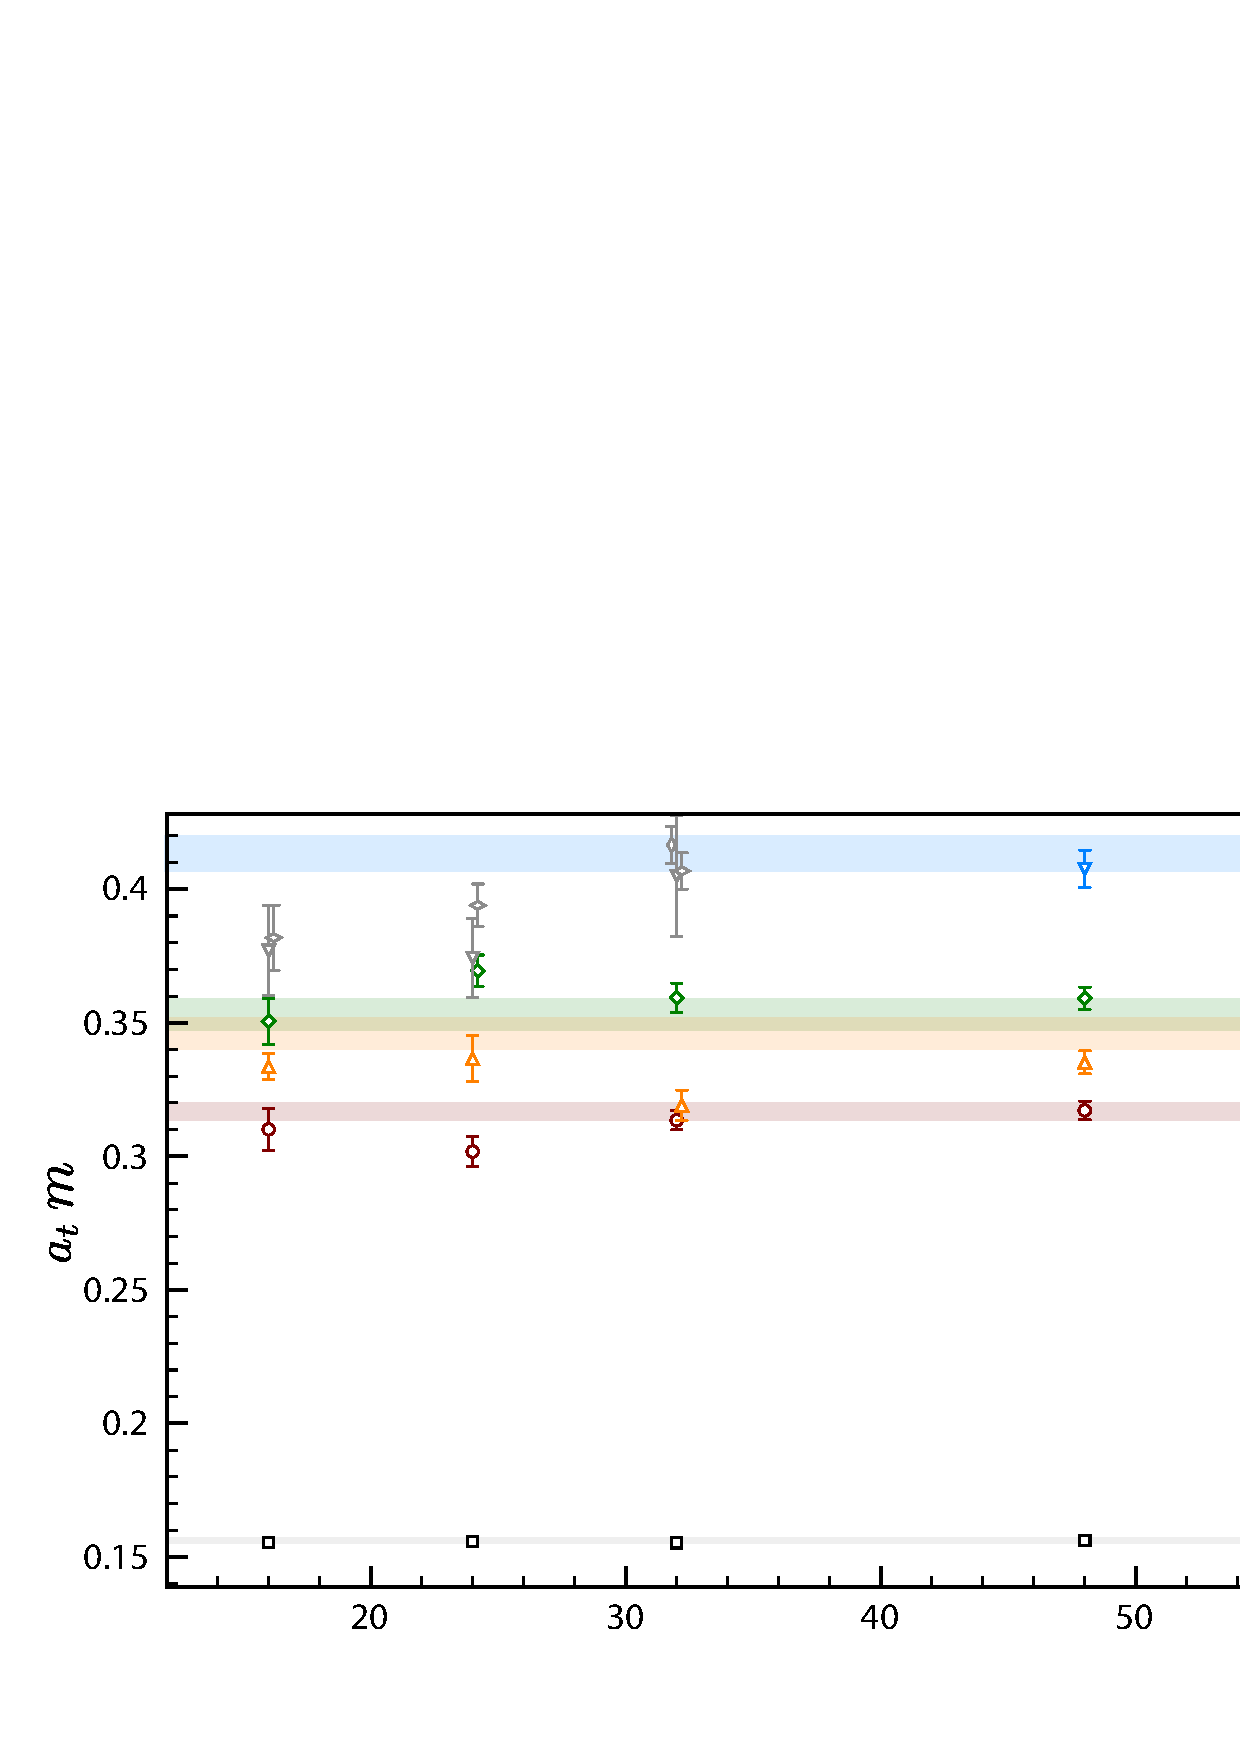
\includegraphics[width=12cm]{images/variational_16.pdf}
\caption{\label{variational} $T_1^{--}$ variational mass spectrum as a
function of number of eigenvectors used. The
error bars are purely statistical and do not take account of possible
systematic errors due to fitting.   }
\end{figure}
Clearly,
even with a relatively small number of vectors this method
can be used to construct two-point correlation matrices from which the
spectrum of low-lying states can be extracted with some precision.
The masses, up through the fourth excited state, become more consistent
with increasing number of vectors.

Now consider the issue of the scaling of this method with increasing lattice
volume. Fig.~\ref{voltest} shows the effective masses of correlators computed
on both $16^3$ and $20^3$ lattices, the spatial-volume ratio here being very
close to 2 ($\tfrac{20^3}{16^3} = 1.95$). It is evident that the
correlation function with $N$ vectors on the $16^3$ volume is essentially the
same as the corresponding case with $2N$ vectors on the $20^3$ lattice. Note
that although the number of inversions for the same signal is doubled when the
lattice volume increases from $16^3$ to $20^3$, there is a reduction in the
noise of approximately a factor of two.

A strikingly simple explanation for this effect comes through consideration of
the eigenvalues belonging to these eigenvectors of the Laplacian operator,
$\nabla^2 v^{(k)} = - \lambda_k v^{(k)}$. Fig.~\ref{evals}(a) shows the
eigenvalues measured on $16^3$ and $20^3$ lattices. One could consider choosing
the rank of the distillation operator by using all eigenvectors with
eigenvalue below a certain
cut-off. It is clear from the plot that on a larger volume this will require
more eigenvectors. This is displayed more directly in Fig.~\ref{evals}(b)
where the number of eigenvectors with eigenvalue less than a cut-off is
plotted. Approximately twice as many eigenvectors in
the $20^3$ case are required to have the same cut-off as in the $16^3$ case.
It appears from this analysis that the meson correlator signal is
effectively determined by the cut-off in eigenvalue used to construct the
distillation space.
This is equivalent to using a Heaviside approximation to smearing:
$J_{\lambda}(t) = \Theta( \lambda + \nabla^2(t)  ) = \sum_{k=1}^M \Theta(\lambda -  \lambda_k )  v^{(k)}(t) v^{(k)\dag}(t) = \sum_{k=1}^{N(\lambda)} v^{(k)}(t) v^{(k)\dag}(t).$



\begin{figure*}
 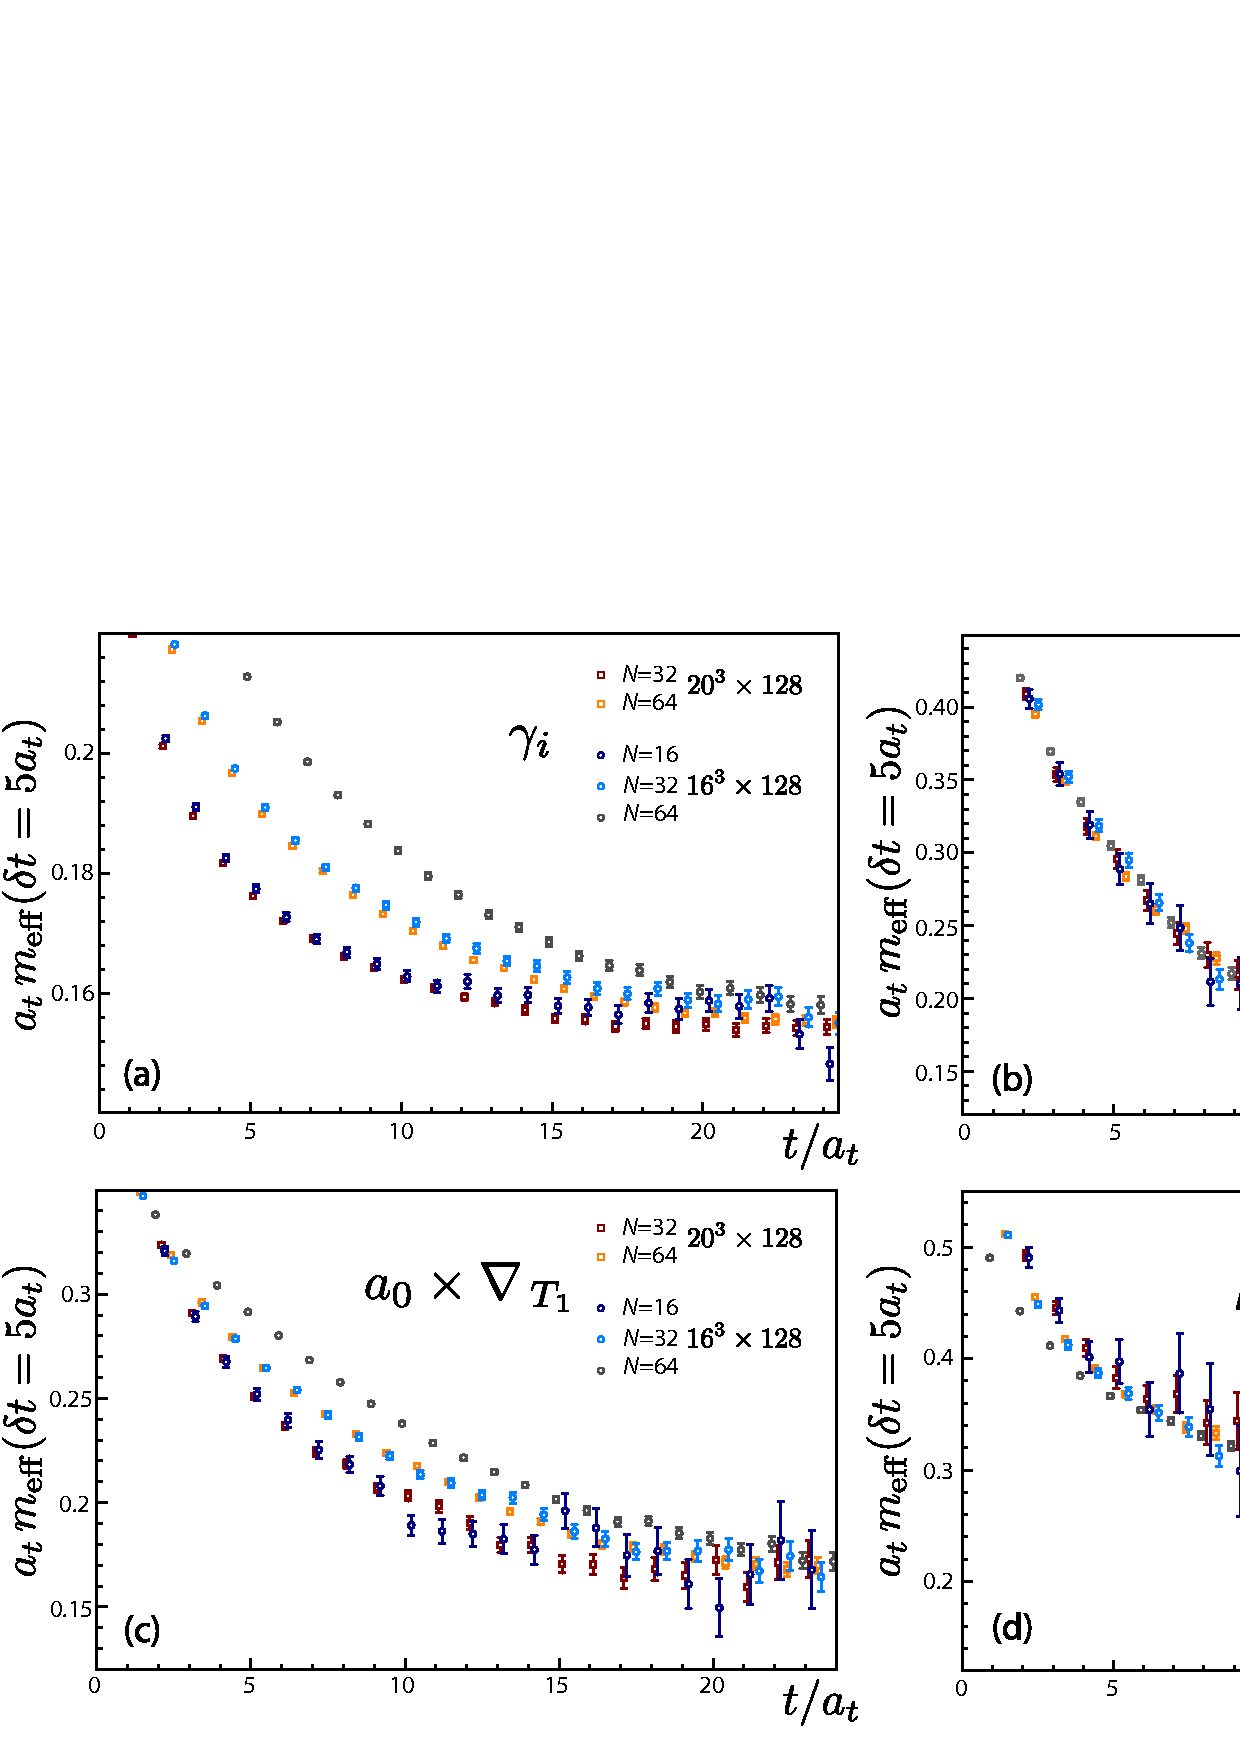
\includegraphics[width=16cm]{images/combined_16vs20.pdf}
\caption{\label{voltest} Effective masses (five timeslice shift) for diagonal correlators in the
$T_1^{--}$ channel on $16^3$ and $20^3$ spatial volumes. Operator construction shown in table
\protect \ref{optab}. }
\end{figure*}

\begin{figure*}
 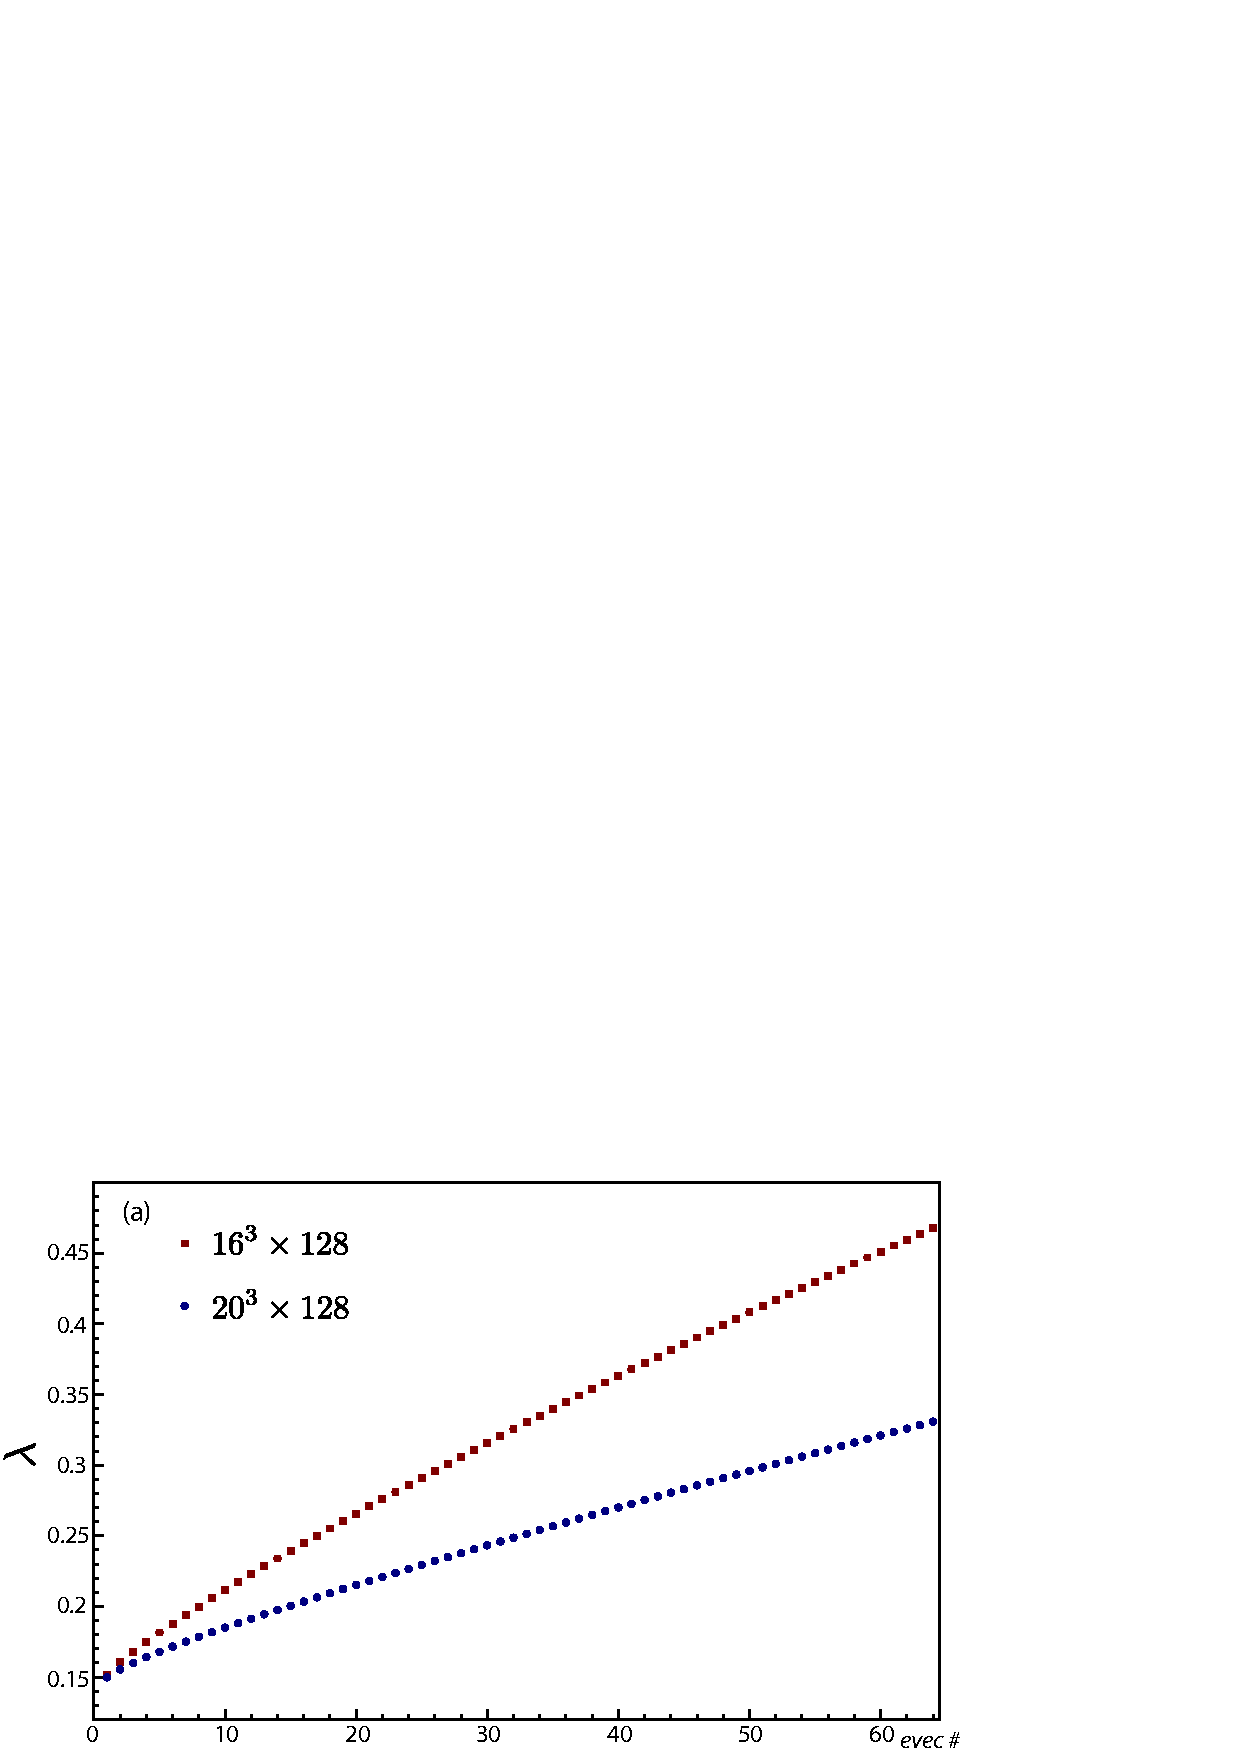
\includegraphics[height=5cm]{images/evals_edited.pdf}
\hspace{5mm}
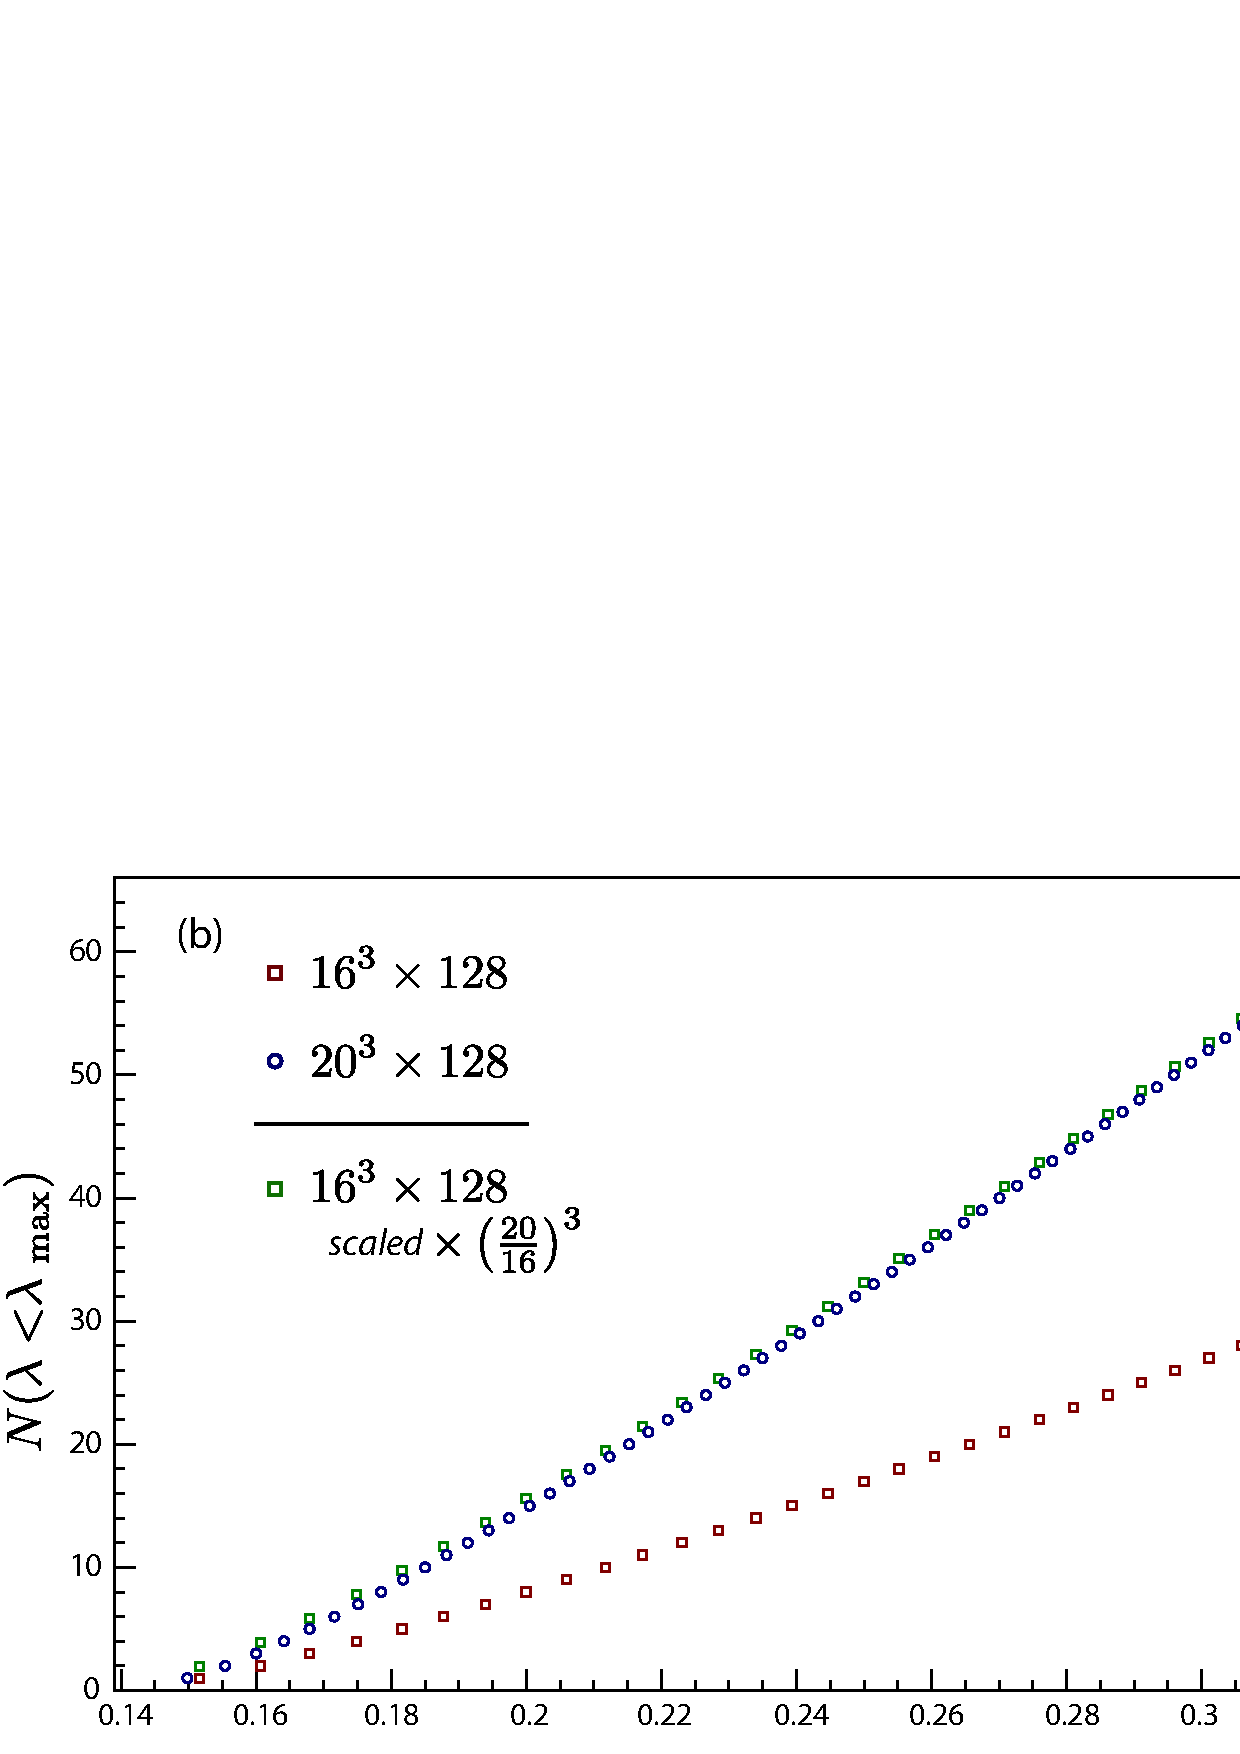
\includegraphics[height=5cm]{images/cutoff_new_edited1p95.pdf}
\caption{\label{evals} (a) Eigenvalues of the laplacian on $16^3$ and $20^3$ lattices. (b) Number of eigenvectors with eigenvalue below $\lambda_{\mathrm{max}}$ on $16^3$ and $20^3$. Also shown is the $16^3$ data scaled by a factor of $\left(\frac{20}{16}\right)^3$.  }
\end{figure*}

\subsection{Baryon correlation functions}\label{subsec:results-baryons}

Baryon correlation functions were evaluated using
the displaced-quark operators described in
Refs.~\cite{Basak:2005aq,Basak:2005ir} and employed in spectrum studies
Refs.~\cite{Basak:2007kj, Bulava:2009jb}.
The distillation method is demonstrated on four nucleon $G_{1g}$
operators, two of which are local to a single site with the remaining two
having a singly displaced quark field. The corresponding $4 \times 4$ matrix of correlators was computed on 316 configurations of the $16^3 \times 128$
lattice. Fig.~\ref{fig:baryon_meff_Nev} shows the effective-mass plots for
the diagonal correlators. A clear trend is observed, similar to that seen for
the mesons, of the correlator having larger excited-state contribution but
smaller statistical fluctuations as the number of eigenvectors is increased.
\begin{figure}
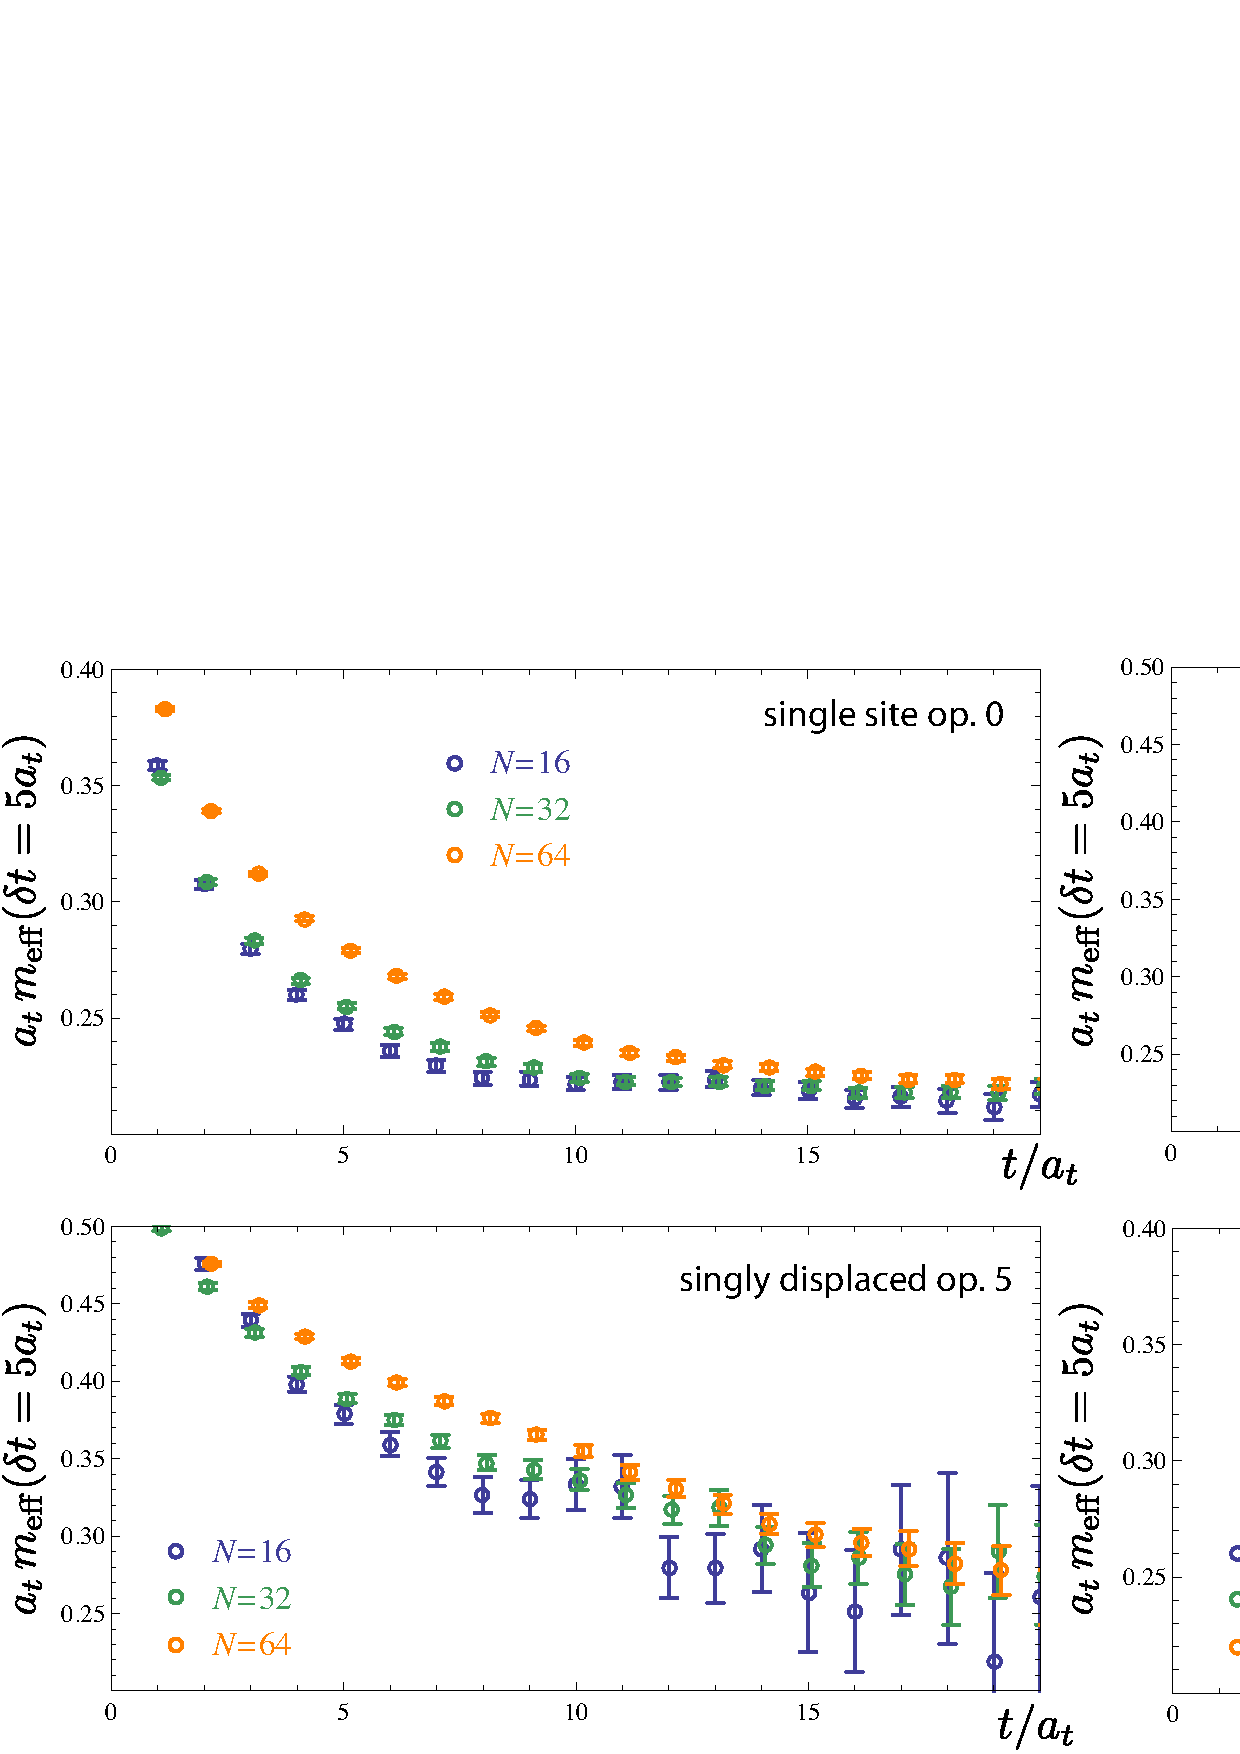
\includegraphics[width=0.9\textwidth]{images/baryon_meff.pdf}
\caption{\label{fig:baryon_meff_Nev}Effective-mass plot for two single-site and two singly displaced operator correlators in the nucleon $G_{1g}$ channel.
}
\end{figure}
Modelling the correlator noise-to-signal ratio with Eq.~\ref{noise}
gives best-fit exponents $p \sim 1.1(2)$, showing again that
increasing the number of vectors decreases the noise considerably faster than
simple statistical scaling.
The variational method \cite{Michael:1985ne,Luscher:1990ck} was used to extract
the masses of the lowest two states in the $G_{1g}$ spectrum.
Fig.~\ref{fig:baryon_Pmeff_Nev} shows the dependence of the effective masses of
these states on the number of eigenvectors used to form the
distillation operator.  Consistent masses are found, with an increase in
statistical precision as the number of vectors is increased.
\begin{figure}
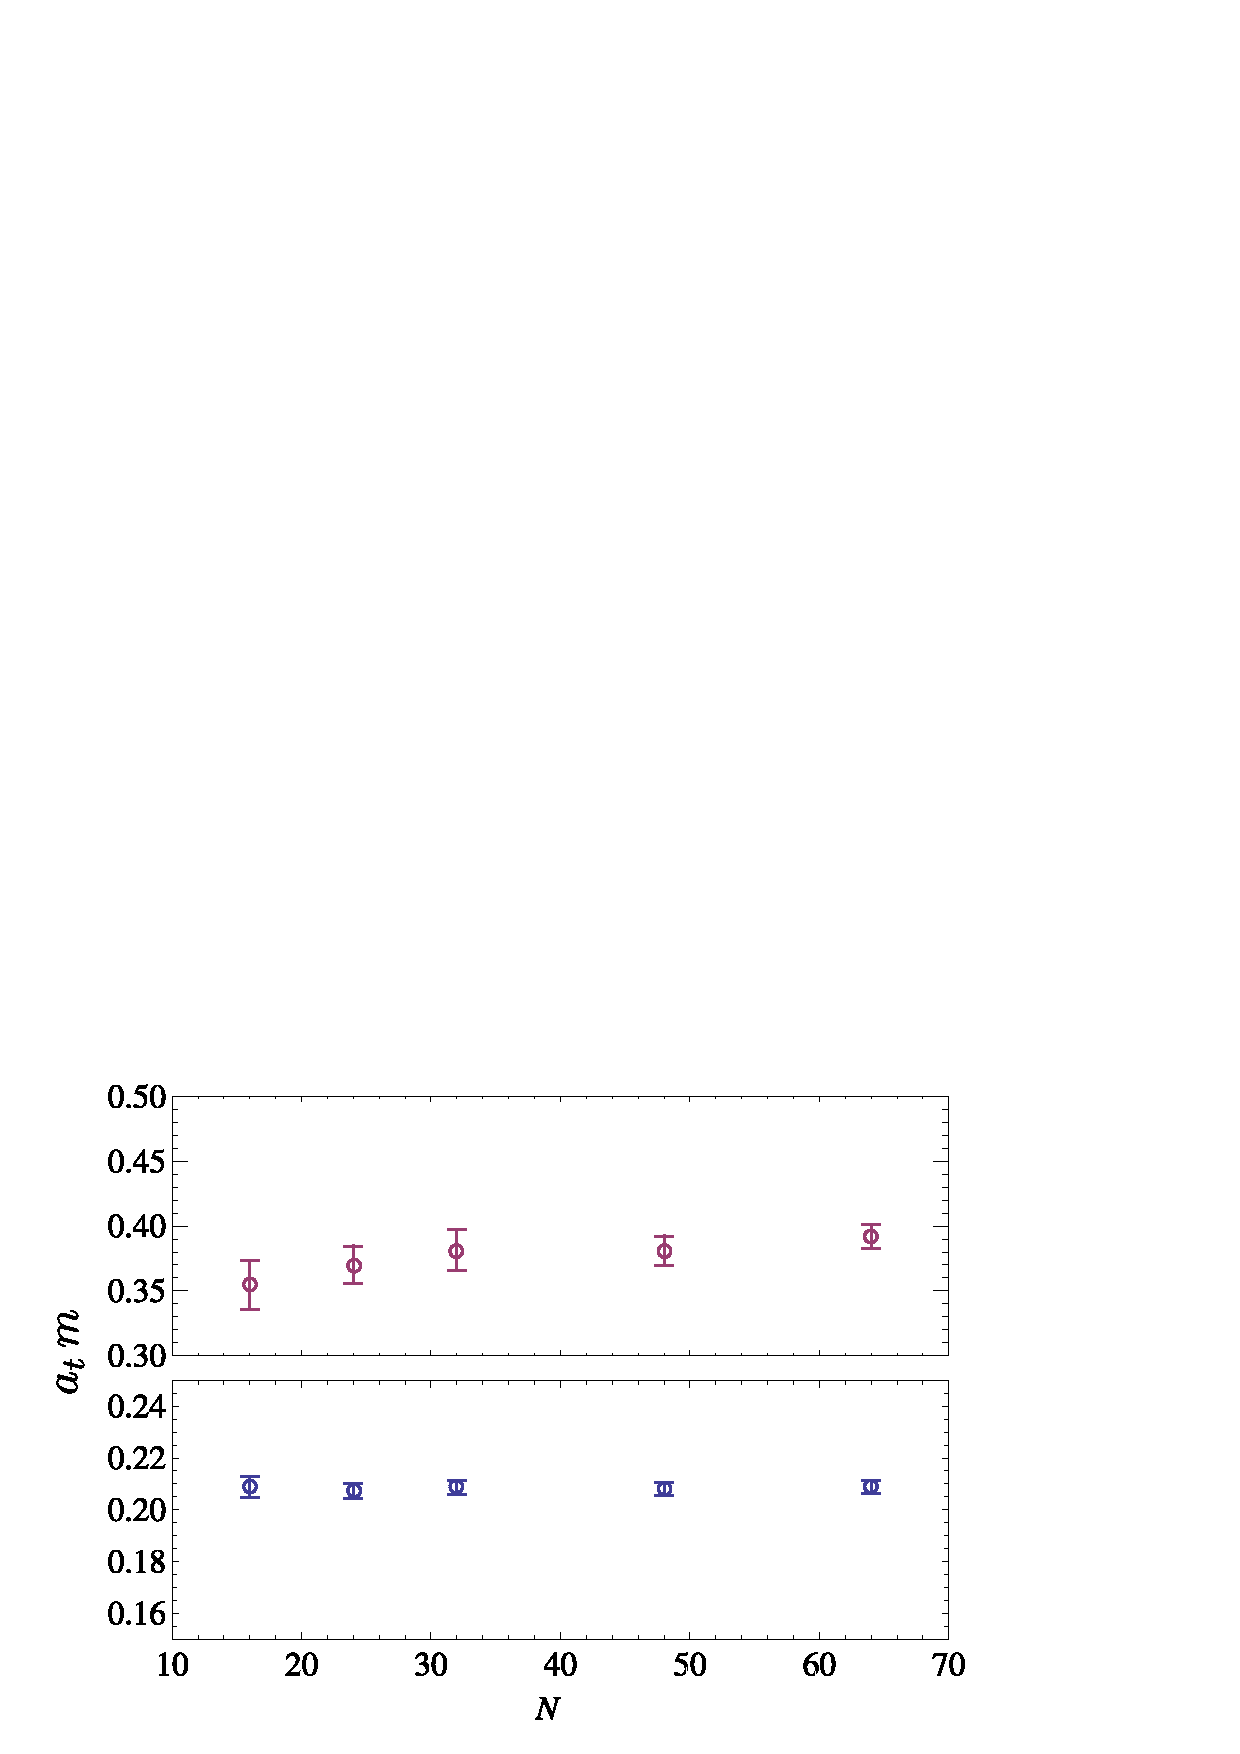
\includegraphics[width=0.5\textwidth]{images/G1g1NevPfitsT07_Ecomp2.pdf}
\caption{\label{fig:baryon_Pmeff_Nev} The fitted energies for the first-excited (top) and ground state (bottom)  as functions of $N$.
}
\end{figure}
Fig.~\ref{fig:baryon_volume_meff_Nev} shows the diagonal effective masses
computed on $16^3$ and $20^3$ lattices.
The similarity between the signals found before and after doubling
the number of vectors is not as obvious here as in the meson case.
\begin{figure}
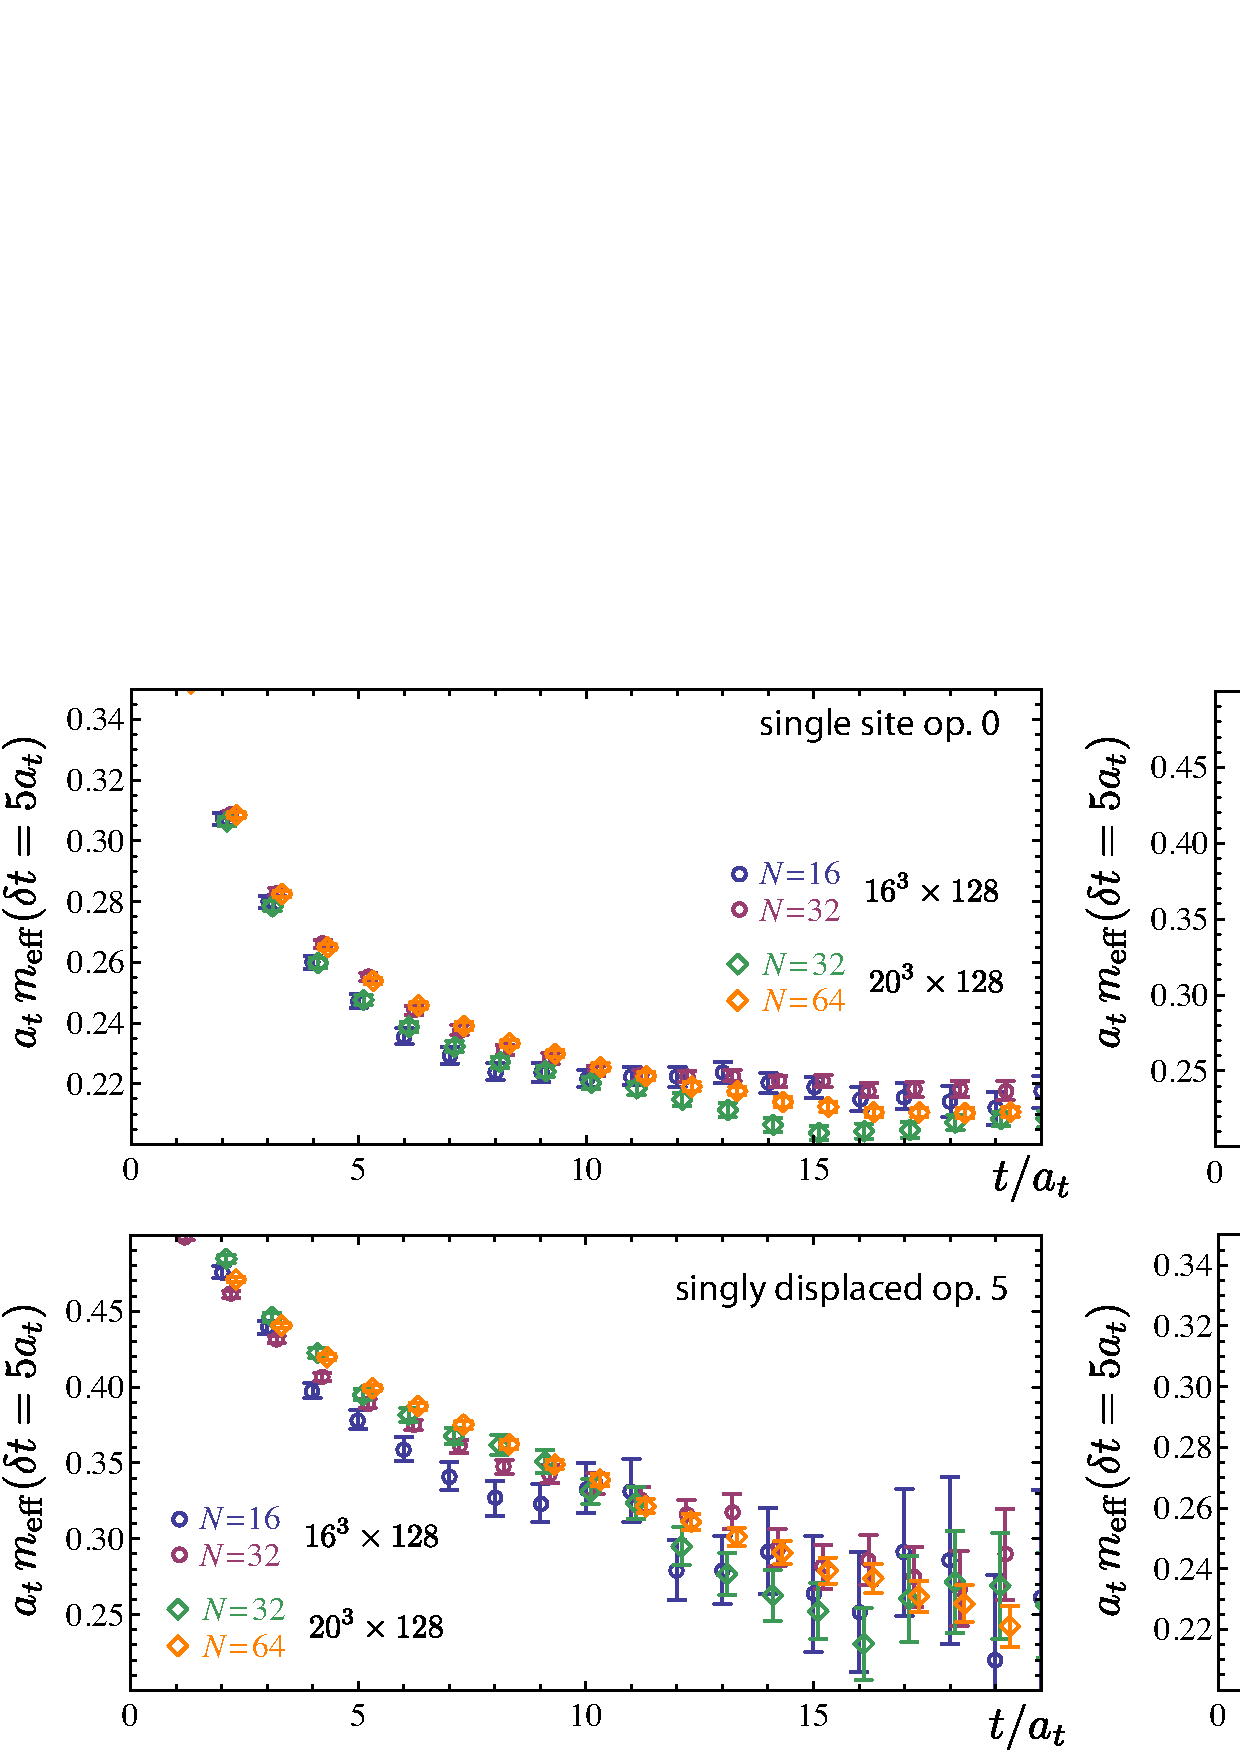
\includegraphics[width=0.9\textwidth]{images/baryon_meff_vol.pdf}
\caption{\label{fig:baryon_volume_meff_Nev}Effective-mass plot for two
single-site and two singly displaced operator correlators from two volumes:
$16^3\times128$ and $20^3\times128$
}
\end{figure}

\subsection{Multi-meson correlation functions}\label{subsec:results-multi-mesons}

One of the main motivations for defining distillation methods is to enable
efficient evaluation of correlation functions of creation operators which
resemble multi-hadron states where the component hadrons have definite
momentum. Reliable and efficient means of including these states in the operator
basis are important for addressing scattering and resonance properties.
The simplest case was tested, which comprises the
isospin-two two-pion state formed using Eq.~\ref{eqn:multi_meson_quark_op} with
the single particle operators $M(\vec{p}_\mathrm{rel})$ constructed using the
local operator $\bar{u}\gamma_5 d$. For this example, consider the
two-pion operator
\begin{equation}
  \chi_{MM}(|\vec{p}_\mathrm{rel}|^2, t) =
    \sum_{k\in {\cal R}(\vec{p}_\mathrm{rel})}
   \chi_M(k,t) \, \chi_M(-k,t)
\end{equation}
with total momentum zero, and the single-particle operators to have relative
momentum $\vec{p}_\mathrm{rel}$. The sum is over the set of momentum vectors
${\cal R}(\vec{p}_\mathrm{rel})$ related to $\vec{p}_\mathrm{rel}$ by lattice
rotations, to create a state that transforms trivially under rotations and so
the operator forms an $A_1$ irreducible representation of the cubic group.
In this test, all values of $|\vec{p}_\mathrm{rel}|$ between 0 and $2 \times
\frac{2\pi}{L}$ were considered, corresponding to $\vec{p}_\mathrm{rel} =
\frac{2\pi}{L}\vec{n}$ with $\vec{n} \in \{(0,0,0), (1,0,0), (1,1,0), (1,1,1),
  (2,0,0)\}$.

A $5\times 5$ correlation matrix is formed between all of these two-pion
operators which
is diagonalized by solving the generalized eigenvalue problem.  The
effective mass of the lowest three principal correlation functions measured on
100 configuration is shown in Fig.~\ref{fig:twopi}. Clear indication of
a signal for the second excited state is seen, even with this relatively
low level of statistics. Note that when using the conventional point-to-all
method, the source operator cannot be projected onto definite momentum so the
correlation matrix described above cannot be constructed in practice.
\begin{figure*}
 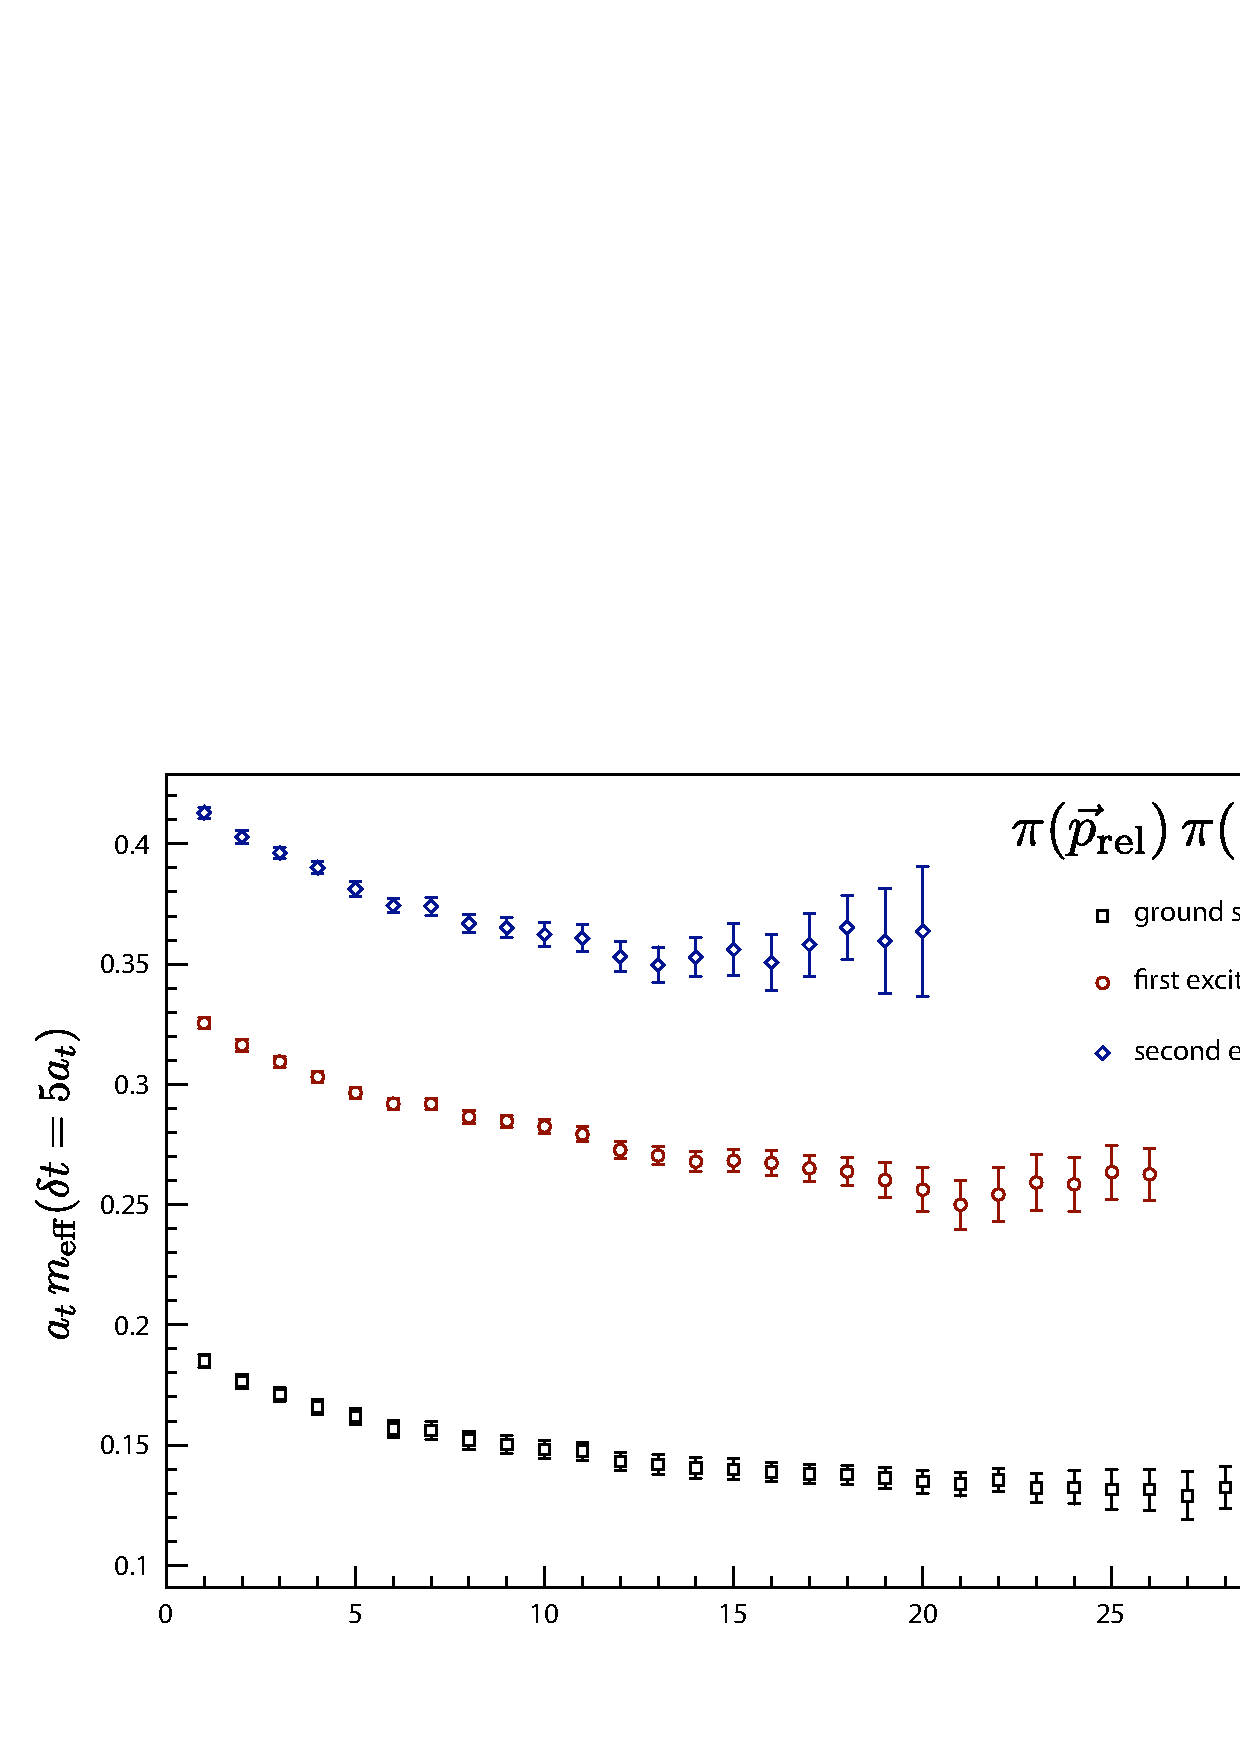
\includegraphics[width=10cm]{images/twopi.pdf}
\caption{\label{fig:twopi} Effective masses (five-timeslice shift) for the first three
principal correlators in the isospin-two $\pi(\vec{p}_\mathrm{rel})\pi(-\vec{p}_\mathrm{rel})$ channel ($A_1^{++}$) computed on
$16^3\times 128$ lattices. The $5\times 5$ correlation matrix
is constructed from $|\vec{p}_\mathrm{rel}|^2 \in [0,4]$.  Correlators constructed
through distillation with $N=64$ vectors on 100 configurations.}
\end{figure*}
